\chapter{Discussion}\label{ch:discussion}
This chapter is based on \cite{Khandelwal2018} and \cite{Hastie2008}.

Some of the models we ended up with, using both $F$-test and cross-validation, included the parameter $cond$.
As it was also mentioned in the introduction, one must be cautious when using a parameter of subjective nature.
Furthermore only 3\% of observations fall in the category ``low'', making this category nearly useless with so few observations.
To make more effective use of a parameter that measure the condition of an apartment it would have been an advantage to have a more objective measure, and also more categories.
The variable we have are, essentially, a binary variable that determines whether the apartment is of ``medium'' or ``high'' condition.

As mentioned in section \ref{subsec:app_of_prediction}, our $year.sale$ coefficients may not be representative of the price trend for a specific year. 
It might therefore have been more useful to treat it as a continuous variable or alternatively split it up into more categories.

At the start of this project many variables were removed and disqualified immediately.
This was because of either incomplete data or presumed little relevance to the price of apartments. 
In the first case, these were potentially relevant parameters, but due to the data collection they were unreliable. 
Either because the NA-values have been distributed systematically or because there were just very few observations. 
The reason for the removal of the remaining variables, was based on a plot with the variable in question and price, to check if there were any immediate patterns.
From this there was made a subjective conclusion of whether or not this influenced the price enough to warrant inclusion in the model. 

Additional variables, such as energy labels or other unmeasured variables almost certainly influence the price as well. 
There may also be immeasurable variables such as the situation of the sellers or how good the local school is.

% \textbf{3 + 5 (Modellering)}
In chapter \ref{ch:likelihood_theory} we concluded that the MLE is efficient and therefore the unbiased estimator that minimizes variance.
There exist regularization, which introduce bias into the regression solution and thereby reduce variance compared to OLS (which under the Gauss-Markov assumptions are equivalent to the MLE).
This is, depending on the method, done by forcing the sum of squared or absolute value of the regression coefficients to be less than a fixed value.
This can then force certain coefficients to be set to zero, effectively choosing a simpler model that does not include those coefficients.
This both makes the model more interpretative and reduces over-fitting/variance.
This simpler model in turn risks under-fitting and thereby more bias.

% It is possible that we may be able to trade some bias for lower variance.
% high bias = under-fitting.
% high variance = over-fitting. 
% irreducible error: noise inherent in the observations.
% Regularization: Reduce variance for OLS, while introducing bias.
% LASSO: 

% \textbf{4 + 6 (Variance/Bias Trade-off)}
Examples of methods that introduce bias with the purpose of lowering variance are ridge- and lasso-regression.
Ridge-regression differs from OLS in that the loss function is not just the $SSR$, as in the case of OLS, but now adds the penalty $\lambda$ times the sum of squared slope coefficients, where $\lambda$ is a tuning parameter.
The tuning parameter value can be determined using $k$-fold cross-validation.
Another similar method is called lasso-regression, here the penalty is $\lambda$ times the sum of absolute slope coefficients.
A significant difference between these two methods, which both uses regularization, is that lasso-regression can eliminate parameters as the coefficients can be 0.
This is not possible in ridge-regression where the coefficients will approach 0.
In relation to subset selection we can view ridge- and lasso-regression as setting a ``soft threshold'' for the parameter whereas subset selection is a ``hard threshold''.
This is because ridge- and lasso-regression penalizes large coefficients whereas subset selection removes parameters completely.

% \textbf{2 (Sammenligning af metoder (svært))}
Throughout this project we have used a variety of methods to design a model that best describes the data in HOME and also best predicts apartment prices given a set of variables. 
We have determined such models using $F$-tests and cross-validation for Copenhagen, Aarhus, Odense and Aalborg.
The two models have come to different conclusions about which model best depicts apartment prices in the four cities. 
The different conclusion from these models is caused by the models different way of functioning, both of which have strengths and weaknesses that influence the result.

The $F$-test test the entire model with all observation in place, and can determine if any of the parameters are insignificant and thus should be omitted.
The $F$-test is sensitive to large sample sizes, where a large $n$ causes the $F$-test to conclude insignificant parameters to be significant. 
This makes the $F$-tests somewhat questionable because of the large dataset. 
Cross-validation, on the other hand, works well with larger datasets because the test data is used to optimize the model. 
% However cross-validation is often performed with a $5$ or $10$ fold which will cause bias.

% Cross-validation is unbiased if the regression is performed $K = n$ times, also known as leave-one-out. 
% When $K = n$ the regression will find the model which explain the test data very precisely but when the model is used on new test data it will have greater variance. 
When $K = 5$ not all the data will be used to explain the test data and thus the estimate will be misplaced, which we here refer to as biased. 
Since the $F$-tests uses the entire dataset when evaluating the model it is unbiased. 
However because this model has a tendency to keep insignificant parameters it is likely to conclude an overfitted model. 
This will cause the model to have more variance and thereby be more unprecise when predicting out-of-sample. 
Cross-validation can be biased for $K = 5$, because the entire dataset has not been used and therefore it will have a higher tendency to conclude an under-fitted model.


% If the cross-validation is performed with $K = n$, then there would be no bias. 
% However the model obtained with $K = n$ would have a higher variance even though this model describes the data very well. 
% For instance if $K = n$ then the chosen model based on the training set will explain the test set very well. 
% However the model will fail to identify which of the relations between the training sets and test data is real and which are noise. 
% Therefore when the training set is to predict another test data it will have a higher variance. 
% In conclusion both $F$-tests and cross-validation has substantial flaws which influence which parameters is included in the final model and therefore the two tests reach different conclusions. 

% \textbf{1 (Metoder i CV (k = n)} \\
As earlier stated in section \ref{sec:CV}, $K = n$ is another common choice for $K$ fold cross-validation also known as leave-one-out cross-validation.
The advantages of this method is that it is far less biased as the entire dataset has been used for training compared to the 5 fold cross-validation.
Here, a subset of only 80\% of the dataset has been used for training.
This issue is expressed in figure \ref{fig:CrossValidationCopenhagen} where each fold obtain different results.

Additionally the model provides no randomness in the test- and training data as the model yields the virtually same result every time.
Each time performing the 5 fold cross-validation yields different result as the test- and training data is chosen randomly.
However, the method has not only advantages compared to the 5 fold cross-validation.
RMSE varies as the testset contains only one observation. 
If the observation is an outlier then the variance will be high.
The method therefore can result in higher variance compared to the 5 fold cross-validation.
Another trade-off is that the execution of the method is more expensive as the model has to be fitted $n$ times.
The leave one out cross-validation is run for the four cities and the result is plotted in figure \ref{fig:cv_k=n}.
\begin{figure}[H]
        \centering
      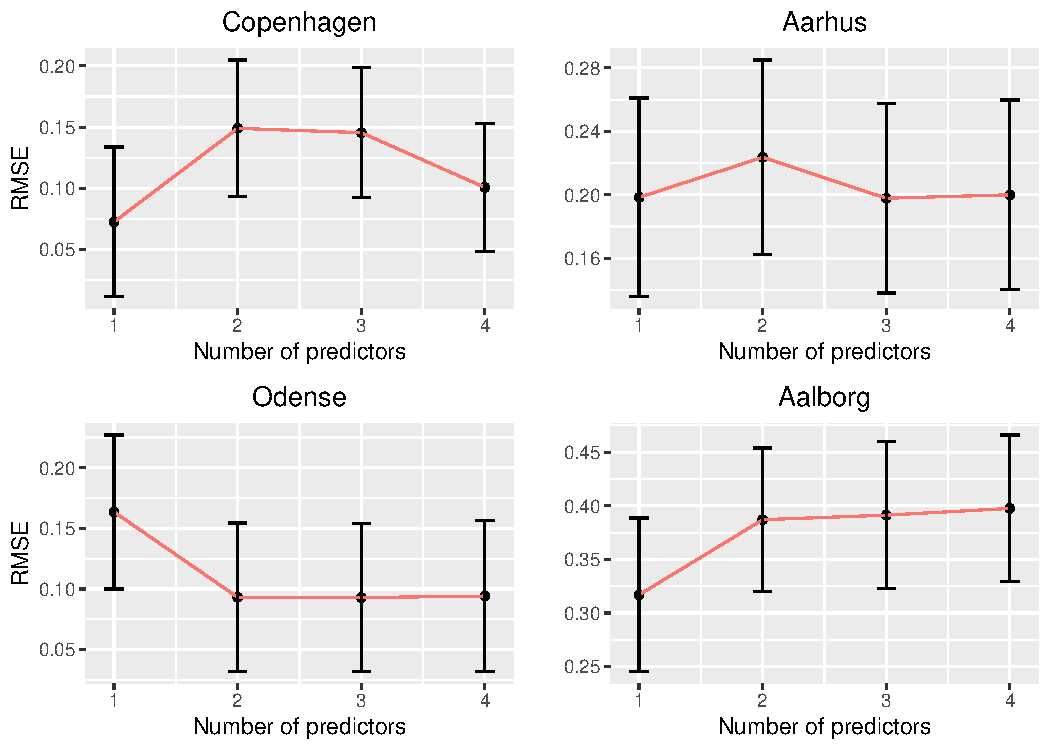
\includegraphics[width = 0.75 \textwidth]{figures/Nanna/k=n.pdf}
      \caption{Result from $K = n$ fold cross-validation.}
      \label{fig:cv_k=n}
\end{figure}
If the figure is compared to the respective figure \ref{fig:CrossValidationSamlet} obtained from 5 fold cross-validation the results are different for every city.
For leave-one-out cross-validation the optimal number of parameters for the four cities is two for Odense and one for the others.
As we obtain different results from the two applications of cross-validation another interesting take on this project would be to compare the two methods with respect to validation and predictive performance.